\documentclass[dvipdfmx,11pt,a4j]{jarticle}  
% qexam_examples.tex - 試験問題の例
% 2009-07-11 Taku Yamanaka (Physics Dept., Osaka Univ.)
% 2019-06-20 Taku: Updated for v2.0.

%-------- page style ----------------------
%\usepackage[a4paper]{geometry}
%\usepackage[a4paper,text={17cm,25cm},centering]{geometry}	% to expand the text area

%\pagestyle{empty}		% suppresses page numbering

%--------- users packages ---------------
%% AMS math package
%\usepackage{amsmath}
%% eps ファイルを読み込むためのパッケージ
\usepackage{graphicx}
%\usepackage{bm} % for vectors in bold math
%\usepackage{udline} % for underlines crossing multiple lines

\usepackage{qexam} %試験問題用パッケージ

%====================================
\begin{document}
%% 和文フォントをゴシック体に変更する。
%% 明朝体でいいときは、コメントアウトする。
%\fontfamily{gt}
%\selectfont
%%%%

%\renewcommand{\questionFormat}[1]{%
%% Here are some examples.  Tune them as you like.
%%	\textbf{\Large{#1}}
%%	\framebox{\LARGE{#1}}
%%	\hspace{-5mm}\textbf{\Huge{[#1]}}
%%	\begin{center}{\textbf{\LARGE{#1}}}\end{center}
%}

%% 問1用のヘディング%%%%%%%%%%%%%%%%%%%%%%%%%%%%%%%%
\begin{center}
	\textbf{\Large  qexam.sty v2.0 を用いた\\
	\bigskip
	試験問題の作成例}\\
	\bigskip
	\textbf{\large 2999年9月9日}
\end{center}

問題1から問題2までのすべての問題に解答せよ。
解答用紙は問題ごとに1枚とし,それぞれに氏名・受験番号・問題番号を書くこと。
%%%%%%%%%%%%%%%%%%%%%%%%%%%%%%%%%%%%%%%%%%%%%

\question{問1}
地の文。
\begin{qlist}
	\qitem 小問
	\qitem 小問
\end{qlist}

\begin{qparts}
	\qpart パート1
		\begin{qlist}
			\qitem 小問
			\qitem 小問
		\end{qlist}
	\qpart パート2
		\begin{qlist}
			\qitem 小問
			\qitem 次の\qbox{(a) -- (b)}を埋めよ。\\
				この \qbox{}埋め 問題に箱は \qbox{}個ある。
		\end{qlist}
\end{qparts}

%end{document}


%% 問題2 %%%%%%%%%%%%%%%%%%%%%%%%%%%%%%%%%%%%%%%
\clearpage
\question{問題2}
問題2の地の文。
問題番号は{\tt \verb"\question{...}"}で指定します。
小問は{\tt qlist}環境の中に{\tt \verb"\qitem"}を使って並べます。

\begin{qlist}

	\qitem 質問その1。
		\begin{eqnarray}
			i \frac{\partial}{\partial t} \psi(t) & = & H \psi(t) \\
									& = & m \psi(t)
%			\nabla \cdot \bm{E}	& = & \frac{\rho}{\epsilon_0}\\
%			\nabla \times \bm{E}	& = & -\frac{\partial \bm{B}}{\partial t}
		\end{eqnarray}

	\qitem 質問その2。図\ref{fig:seagull}に示す、鳥に働く力を考えよう。
		図\ref{fig:seagull}や表\ref{tab:macros}のように、キャプションの数字の後にコロン(:)が入りません。
		\begin{figure}[htbp]
			\begin{center}
				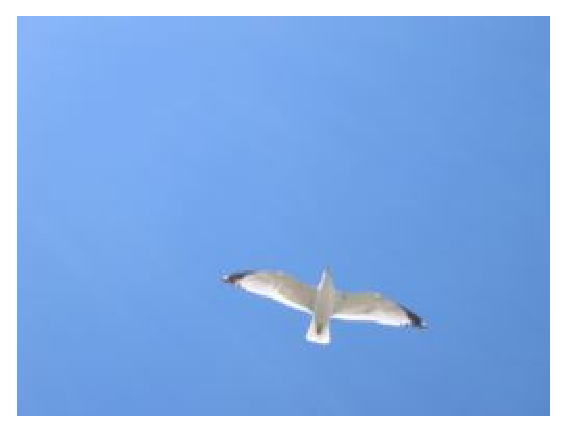
\includegraphics[width=0.3\linewidth]{seagull2.eps}
				\caption{\label{fig:seagull}}
			\end{center}
		\end{figure}

		\begin{table}[htbp]
			\centering
			\caption{\label{tab:macros}}
			\begin{tabular}{|c|c|}
				\hline
				問題 & マクロ\\
				\hline
				大問	& \verb"\question{...}"\\
				中問 & qparts環境の中の\verb"\qpart"\\
				小問	& qlist環境の中の\verb"\qitem"\\
				微小問 & qlist2環境の中の\verb"\qitem"\\
				穴埋め & \verb"\qbox{}"\\
				\hline
			\end{tabular}
		\end{table}
	
	\qitem 質問その3。さらに細かな質問をする場合、{\tt qlist2}環境を使います。
		\begin{qlist2}
			\qitem 微小問題1
			\qitem 微小問題2
			\qitem 爆笑問題3
		\end{qlist2}
\end{qlist}

%% 問題3 %%%%%%%%%%%%%%%%%%%%%%%%%%%%%%%%%%%%%%%
\clearpage
\question{問題3}

問題3の地の文。中問がある場合は、{\tt qparts}環境を使います。

\begin{qparts}
	\qpart まず、フォースが働かない場合を考えよう。
		\begin{qlist}
			\qitem Yodaにかかる力を図示せよ。
			\qitem Lukeが宇宙船に及ぼせる力の上限を求めよ。
		\end{qlist}
        
	\qpart 次に、フォースが働く場合を考えよう。
		\begin{qlist}
			\qitem \label{q:forcerange}
				フォースの距離依存性を式で表せ。
			\qitem Lukeが宇宙船を持ち上げることができるか、
				\qref{q:forcerange}の結果を元に計算して求めよ。
				
				このように、{\tt \verb"\label"}と{\tt \verb"\qref"}を
				用いて小問の参照もできます。
	        \end{qlist}
	        
	        中問{\bf II}の中の地の文。
	       このように、小問の番号は、中問が変わっても連続した数が割り振られます。
\end{qparts}

\bigskip
さて、がらりと舞台は変わって10次元の宇宙では....というように
中問と中問の間に問題2の地の文を入れることもできます。

\begin{qparts}
	\qpart まず、10次元のラグランジアンを考えよう。
		\begin{qlist}
			\qitem 10次元のベクトルを2次元の紙に図示せよ。
			\qitem 小問の番号は、{\tt qparts}環境が途切れても連続します。
		\end{qlist}

\end{qparts}

%% 問題4 ... %%%%%%%%%%%%%%%%%%%%%%%%%%%%%%%%%%%%%%%
\clearpage
\question{〔4〕}

穴埋め問題には\texttt{qbox}を用います。
次の\qbox{(a)}から\qbox{(b)}に当てはまる式を答えよ。

\begin{qlist}
	\qitem 静止している質量$m$の粒子の全エネルギーは$E = mc^2$であるが、
		粒子が速度$\beta = v/c$で動いている場合、粒子のエネルギーは
		ローレンツファクター $\gamma =\ $\qbox{} を用いて \qbox{}と表される。
\end{qlist}
%% 問題5 ... %%%%%%%%%%%%%%%%%%%%%%%%%%%%%%%%%%%%%%%
\clearpage
\questionNoSkip{5.カスタマイズ}
様々なカスタマイズもできます。
\verb"\questionNoSkip{}"を用いて、改行せずに問題の地の文を続けたり、

\verb"\questionFormat"コマンドを定義し直して大問の形式を変えて

\renewcommand{\questionFormat}[1]{%
% Here are some examples.  Tune them as you like.
%	\framebox{\LARGE{#1}}
%	\hspace{-5mm}\textbf{\Huge{[#1]}}
%	{\Large 〔{\gt \arabicz{#1}}〕}~%
	{\Large 〔{\gt #1}〕}~%
}
\question{5}
問題番号を大きくして鍵括弧でくくったり、

\renewcommand{\questionFormat}[1]{%
	\begin{center}{\textbf{\LARGE{#1}}}\end{center}
}
\question{問題6}
中央に置いたり。

\begin{qparts}
	\qpart 中問のフォーマットも\verb"\qpartFormat"を定義し直せば変えられます。

	\renewcommand{\qpartFormat}[1]{%
		\item [\LARGE{\textbf{\Alph{#1}}.}]
	}
	\qpart \arabic{qpartNumber}番目の中問を大文字のアルファベットで表すと\Alph{qpartNumber}。

	\qpart 小問、微小問のprefix
		小問や微小問の問題番号の前に文字列 (prefix)を入れることもできます。

		\begin{qlist}[小問]
			\qitem 小問には{\tt \verb"\begin{qlist}[...]"}で指定。
			\qitem 微小問には{\tt \verb"\begin{qlist2}[...]"}で指定。
				\begin{qlist2}[case ]
					\item 宇宙が膨張する場合。
					\item 宇宙が収縮する場合。
				\end{qlist2}
				
			\qitem 微小問に小問の番号をつけ加えるには{\tt \verb"\begin{qlist2}[\arabic{enumi}-]"}で。
				\begin{qlist2}[\arabic{enumi}-]
					\item どや
					\item でや
				\end{qlist2}
		\end{qlist}
		
	\qpart もっと大幅に小問のフォーマットを変えるなら\verb"\qitemFormati"、
		微小問のフォーマットを変えるなら\verb"\qitemFormatii"を定義し直します。
		\renewcommand{\qitemFormati}[1]{%
			\textbf{問 \arabicz{\arabic{enumi}}}
		}
		
                \renewcommand{\qitemFormatii}[1]{%
                		\textbf{微小問 #1\arabic{enumii}}
                }
                
                \begin{qlist}
                		\qitem 括弧がなくなったし
			\qitem \verb"\arabicz"を用いると全角数字に
				\begin{qlist2}
					\qitem こちらは括弧なしの半角数字に
				\end{qlist2}
                \end{qlist}

	\renewcommand{\qpartFormat}[1]{%
		\item [\LARGE{\textbf{\arabic{#1}}.}]
	}

\addtolength{\qpartMargin}{5mm}
	\qpart スペースを変更する。
		\addtolength{\qlistTopMargin}{-7mm}
		\addtolength{\qlistBottomMargin}{-7mm}
		
		\begin{qlist}
			\qitem 各中問の始まる前のスペースは{\tt \verb"\qpartMargin"}で変える。
			\qitem {\tt qlist}の前のスペースは
					{\tt \verb"\qlistTopMargin"}で変える。
			\qitem {\tt qlist}の後のスペースは
					{\tt \verb"\qlistBottomMargin"}で変える。
		\end{qlist}
	\qpart 図やのキャプションのフォーマットを変える。
		\begin{qlist}
			\qitem 図\ref{fig:standard}のように、キャプションを標準に戻すには
				{\tt \verb"\qUseStandardCaptions"}を使う。
				
				\qUseStandardCaptions
				\begin{figure}[htbp]
					\begin{center}
						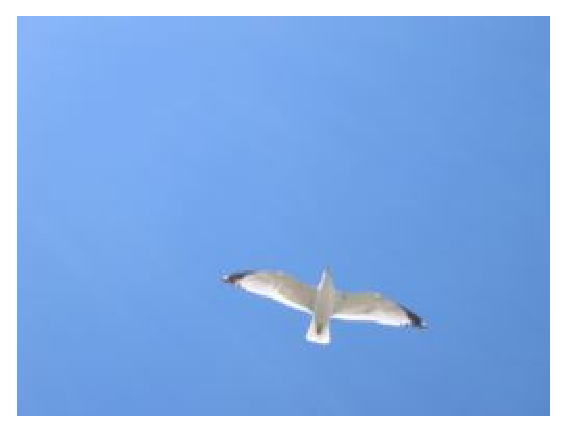
\includegraphics[width=0.3\linewidth]{seagull2.eps}
						\caption{コロンが入っている。}
						\label{fig:standard}
					\end{center}
				\end{figure}
				
			\qitem キャプションをコロン抜きに戻すには
				{\tt \verb"\qUseNoColonInCaptions"}を使う。
				
				\qUseNoColonInCaptions
				\begin{figure}[htbp]
					\begin{center}
						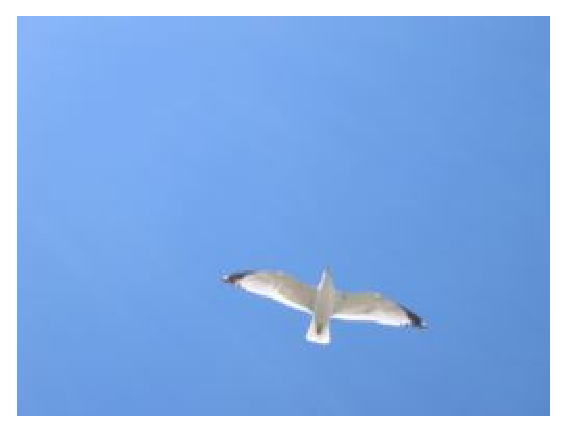
\includegraphics[width=0.3\linewidth]{seagull2.eps}
						\caption{\label{fig:nocolon}}
					\end{center}
				\end{figure}
		\end{qlist}
		


\end{qparts}
\end{document}

